\chapter{背景知识介绍}
\label{chp:background}

随着人们对电子产品的焦点从桌面端慢慢转移到移动端,互联网黑灰产业也有向移动端趋向的迹象。
本章将按自底向上的顺序,分别介绍Android应用程序、应用市场和移动黑灰产相关的背景知识,以期让读者对移动黑灰产的整体生态有大致的了解。

\section{Android应用程序的构建与签名}

Android应用是移动黑灰产的终端环节之一,了解Android应用的构建和签名过程能帮助我们了解黑灰产从业者可以在哪一步植入牟利手段。

\subsection{Android应用程序构建}

与大部分软件一样,开发者在发布自己的App之前,也先需要把代码编译打包成Android操作系统使用的一种应用程序包格式文件,即APK(Android application package)。
每个APK文件都会包含该款App的一系列基本信息,包括App的应用名、包名(Package name)、安全证书等。
其中,包名是Android系统识别App的依据,每款App在不同的版本可以有不同的应用名,但其包名必须是一致的。
\autoref{fig:Android-Build-Process}展现了APK文件的构建流程。
一般来说,一个Android App的构建流程会分为以下四步,整个构建流程由Android SDK中的Android插件和Gradle构建工具管理。

\begin{figure}[htbp]
	\centering
	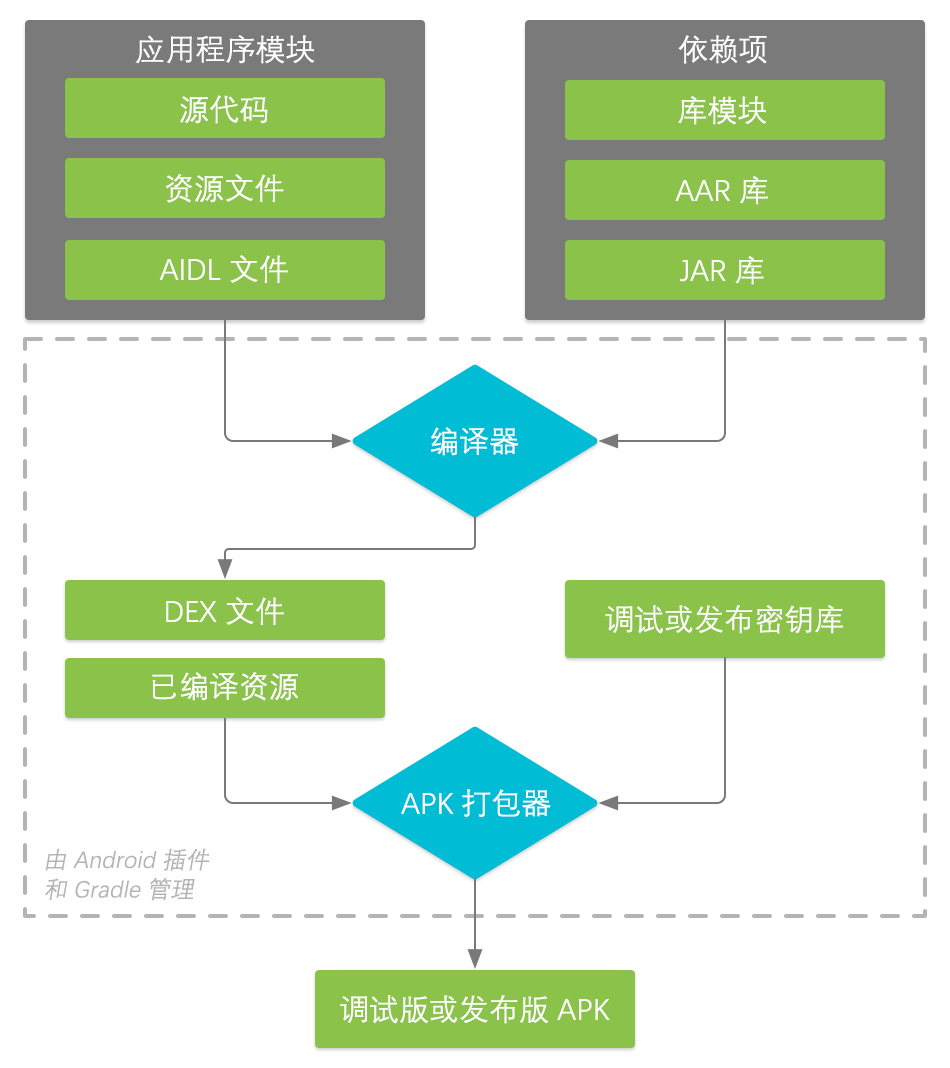
\includegraphics[width=0.6\textwidth]{./Figures/edwin-build-process-CHN.png}
	\caption{Android App构建流程}
	\label{fig:Android-Build-Process}
\end{figure}

首先,开发者需要编写App对应的源代码,然后连同一些源代码中使用到的依赖项一起输入到编译器中生成DEX文件。
源代码可以由Java语言或者Kotlin语言编写,而DEX文件则是一种可执行文件,可以运行于Dalvik虚拟机上。
Dalvik虚拟机则是Android系统的核心组成部分之一,用于运行被编译为DEX文件的程序。
此外,编译器还会将其他未被编译的资源文件转换为编译后的资源。
黑灰色产业从业者可以在这步就将恶意代码植入到应用中。

然后,SDK中的APK打包器会将DEX文件和已经编译好的资源文件一起打包。
APK文件的本质是压缩文件,其中包含了被编译的代码文件、App需要用到的资源文件(比如字符串、图片等资源)、assets资源、App的安全证书和Manifest配置文件,所以APK打包器的任务是将这些所有文件都压缩进一个APK文件里面。
不过,在这个步骤,APK打包器还未将所有文件压缩。
因为在压缩之前,还需要进行下一步的签名。

在第三步,APK打包器会使用密钥库文件对上一步中提及的资源文件和代码文件进行数字签名。
这个步骤是用作校验APK文件是否被篡改、保证APK文件完整性的一个重要步骤,但也是黑灰色产业从业者可以利用的一个环节。
下一小节会有相关机制的更多介绍。

最后,APK打包器会使用zipalign工具对应用进行优化,以减少App在设备上运行时所占用的内存。
这步结束之后,整个构建流程也随之结束。
开发者会获得一个编译好、签名完毕并且经过优化的APK压缩文件,然后就可以将这个APK文件安装到Android设备上运行使用。

目前,随着技术发展,互联网上还出现了各式各样的App生成器~\cite{anjian, iApp},用户无需了解复杂编程知识,只需简单操作即可实现App的开发。
一方面,这种简易的开发步骤有助于黑灰产从业者快速生产恶意应用;
另一方面,App开发框架的提供者本身也可能对生产出的App嵌入恶意代码。
业界相关报告~\cite{anquanke_framework}表明,黑灰产从业者对App生成器的滥用已经带来了严重的安全隐患。

\subsection{Android应用签名机制}
\label{sec:signature}

开发者在使用Android SDK构建App时,其中十分重要的一步是对App进行数字签名。
实际上,Android的数字签名和安全证书机制基于RSA公共密钥系统,是Android安全机制中不可或缺的一个部分。
本章的余下内容将会对Android App的签名机制进行简单分析。

Android App的签名机制是用作校验APK文件是否被篡改、保证APK文件完整性的一个重要机制,所有的应用都必须要在经过签名才能安装进Android系统中。
在签名时,SDK会使用一种密钥库文件,如果开发者还没有这个文件的话,SDK会自动生成一个。
密钥库中包含了开发者的各种信息,包括一对公钥和私钥。
私钥用于数字签名,不可向外公布;公钥则是可以向外公布的一组密钥,用于数字前面的验证。
App中的签名也是系统用来识别开发者的重要依据,因为同一个密钥库文件会产生一致的签名,系统能根据签名中的公钥验证应用识别开发者。

签名的过程大致如下:
在前文流程的第二步结束后,编译器会输出DEX文件和编译好的资源文件,这时,SDK会对每个文件都扫描一次,然后对每个文件提取一次数字摘要,再把每个文件的文件名和其对应的数字摘要保存在一个名为\textit{MANIFEST.MF}的文件中。
之后,SDK会再扫描一次刚才生成的\textit{MANIFEST.MF}文件,再次提取一次数字摘要,把这个摘要连同刚才文件中的所有内容存入另一个新文件\textit{CERT.SF}里。
第三步,再计算一次\textit{CERT.SF}的数字摘要,然后用密钥库中的私钥对这个摘要进行加密。
加密后的结果就是数字签名。
最后,SDK将签名、公钥、计算数字摘要的哈希算法等信息写入\textit{CERT.RSA}文件中,再将这整个过程中生成的四个文件放进\textit{META-INF}文件夹,用APK打包器打包起来。
至此流程结束。

而Android系统验证签名的方式,则是先通过\textit{CERT.RSA}中的公钥验证签名是否无误,再根据文件中提供的哈希算法计算APK包中所有文件的数字摘要:先从\textit{CERT.SF}开始,然后是\textit{MANIFEST.MF},然后是APK中的其他所有文件...
一旦其中出现不相符的结果,就会导致验证失败。
在安装App的过程中,验证签名失败会使得系统终止App的安装。

换句话说,在一个APK被打包签名完毕之后,如果需要更改其中的内容,就只能在更改后将APK重新打包签名一次,即使是一个bit的修改也会破坏原有的签名。
这也是系统可以用数字签名识别开发者的原因:签名一致的App,最后一定都是由同一个开发者打包的。
所以,具有同样签名的App也可以在同一个Android设备上共享数据。
不过这超出了本文讨论的内容,故按下不表。

目前,签名的模式共有三代,其区别主要在于构建流程第三、第四步之间的一些操作上。
简单地说,越新的签名模式能越好地保障APK文件的完整性。
实际上,第一代签名模式V1具有较为致命的缺陷,所以Google官方也在呼吁开发者在编译时采用最新的签名模式。

要注意的是,签名机制只能保证APK文件在被篡改之后不能凭借原有的签名被安装进Android系统,但恶意开发者依然可以在篡改APK之后,用自己的密钥库对APK重新签名,构建出可安装的App。
这种App是盗版App的一种,被称为重打包App。

另外,虽然一个安全证书只能指向一名开发者,但一个开发者可以同时拥有多个安全证书。
开发者和安全证书之间具有一对多的映射关系。

\section{Android应用市场}
\label{sec:androidMkt}

由于每个人都可以开发、构建自己的Android App,从网上发布的App数不胜数。这种开放性为Android应用生态带来开放性的同时,也会引入包括安全隐患等一系列问题。
而Google提供的Google Play应用商店无疑为用户和开发者都提供了一个优良的解决方案。
官方对上架前的应用审核,为用户安全提供了一定保障;商店中每个应用底下由用户评论组成的社区也促成了用户和开发者之间的交流,用户反馈直接推动了开发者对应用的改良。

遗憾的是,由于种种原因,Google Play应用商店的服务并非对全球的所有地区和国家都开放。
Google从2008年开始退出中国大陆市场,因此Google的大部分服务,包括Google Play应用商店的下载服务在内,都不向中国大陆境内用户提供。
换句话说,国内的大部分普通用户并不能享受到Google Play应用商店的便利。

为此,国内有多家厂商都推出了自己开发的应用市场服务,如腾讯旗下的应用宝~\cite{Myapp}和百度旗下的百度应用市场~\cite{Baiduappstore},还有华为的应用市场、小米的小米应用市场~\cite{Xiaomiappstore}等,试图填补这一片市场空白。

\begin{figure}[h]
	\centering
	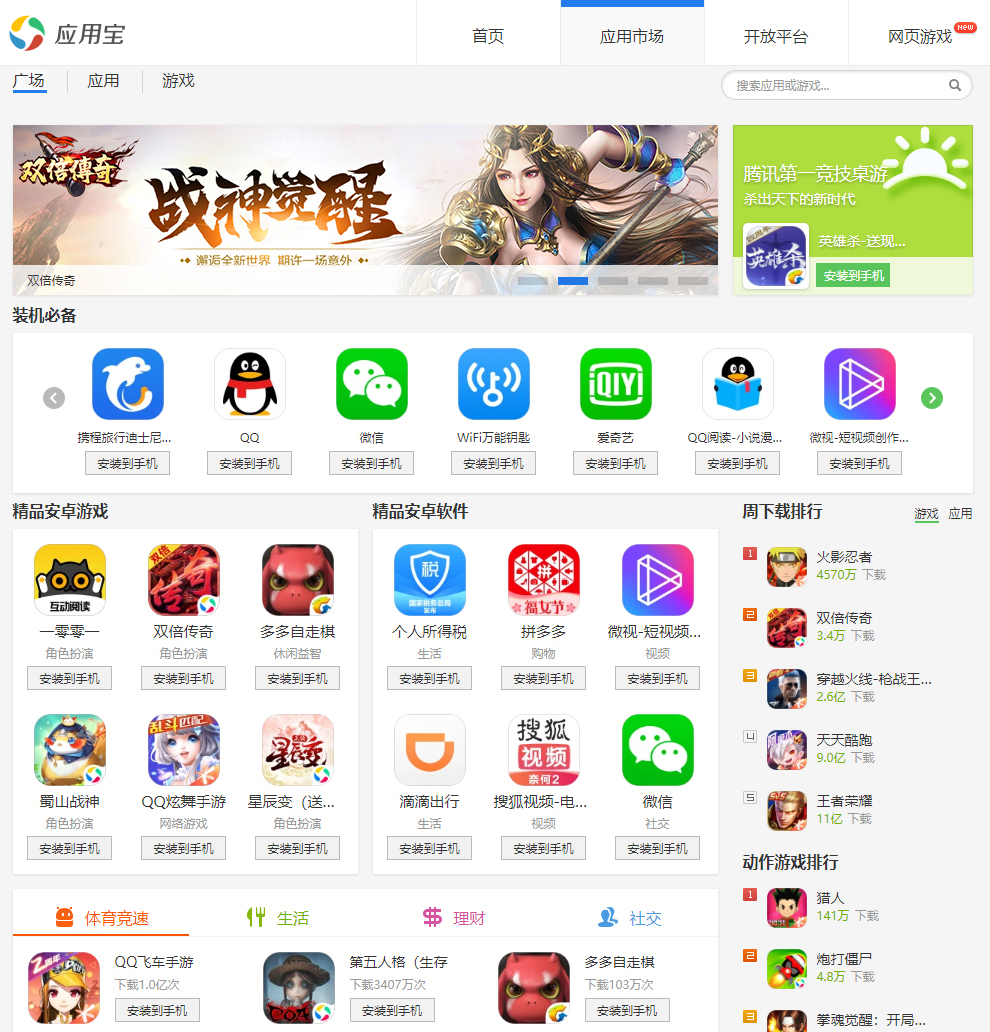
\includegraphics[width=0.8\textwidth]{./Figures/edwin-yyb.jpg}
	\caption{腾讯应用宝应用市场首页(从桌面端浏览)}
	\label{fig:mkt-yyb}
	\vspace{-5mm}
\end{figure}

不同于在Android系统发布早期就存在的Google Play应用商店,国内的第三方应用商店是后期出现的产物,一出现就面临着激烈的市场竞争。
一方面,在国内各类第三方应用市场方兴未艾之时,国内的Android开发者社群尚未成熟,应用市场还未有大量开发者进驻;
另一方面,在成立初期,为了抢占市场份额,各个应用商店都想方设法将商店内App的种类和数量最大化,以迎合市场用户各种各样的需求。
作为结果,各类第三方应用市场都在各个渠道搜集App,而非通过开发者上传的方式获得货架上的应用程序。
由于在早期各种监管渠道、审核机制尚未完善,各个市场在搜罗各类App的同时,难免会将大量的盗版、恶意应用也一并收录。
换句话说,早期的各类第三方市场为移动黑灰产的成长提供了良好的温床。

\section{移动黑灰产简介}
依托Android端应用进行牟利的移动端黑灰色产业链条多种多样,在此我们向读者介绍与本次研究较为相关的两种:恶意应用与排名欺诈。

\subsection{恶意应用}
恶意应用是移动端黑灰色产业中最重要的一环。
作为与用户接触的终端,恶意应用也是多种形式的黑灰色产业的负载触发点。

要了解恶意应用产业,可以从三个问题下手:
恶意应用是怎么安装到用户的设备里的?
恶意应用都会有什么恶意行为?
这些恶意行为是如何触发的?

1)\ \emph{恶意应用的安装} \quad
相关研究~\cite{Zhou2012DissectingAM}表明,恶意软件的安装途径主要可以分为三个分类:重打包、更新攻击和路过式下载(Drive-by Download)。

重打包的概念在\secref{sec:repackaging}已经有所介绍。
为了诱使用户下载重打包后的应用,黑灰产从业者往往会选择热门的应用进行重打包,再在监管力度不太严格的应用市场进行重新发布。
这意味着,在我们的研究主体——仿冒应用——中,会有一部分重打包应用。
但是,迄今并没有相关研究揭示仿冒应用中重打包应用的占比,我们将在后文进行研究。

更新攻击是指恶意应用开发者为了躲避应用市场的监管审查,有意在应用市场上上架不包含恶意代码的应用,然后在用户安装应用之后,提示用户升级,进而绕开应用市场,将带有恶意代码的``新''版本安装到用户设备上的行为。
\autoref{fig:update-attack}给出了一个更新攻击的样本示例,图片引自Zhou与Jiang于2012年发布的研究~\cite{Zhou2012DissectingAM}。

\begin{figure}[h]
	\centering
	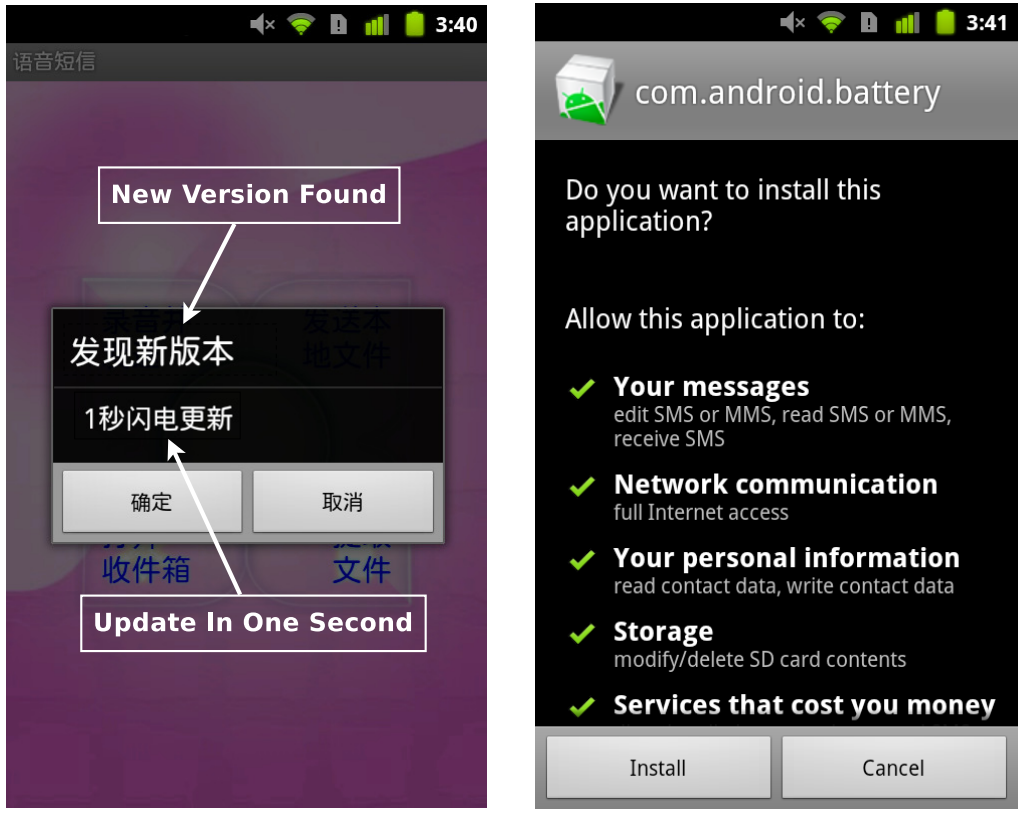
\includegraphics[width=0.7\textwidth]{./Figures/edwin-update-attack}
	\caption{更新攻击样本示例}
	\label{fig:update-attack}
	\vspace{-5mm}
\end{figure}

比起上述的两种安装途径,路过式下载更加隐秘。
路过式下载指在用户不知晓的情况下下载和安装恶意软件,和更新攻击相似,路过式下载行为的携带者(也就是一个表面上没有恶意代码的应用)可以被正常地上传到应用商店中,供用户下载。
等用户安装了对应应用之后,就有可能因为各种事件触发路过式下载,将不想要的应用甚至其他恶意应用静默安装到设备上。
这些事件可以是误触了应用中的某个弹窗广告,也可以仅仅是打开了无线网络开关,路过式下载甚至可以发生在设备每次启动完毕的时候。

2)\ \emph{恶意行为分类} \quad
恶意应用包含的恶意行为同样具有多样性。
以对设备侵入性从高到低排序,已知恶意行为可以被分为几个分类:特权提升,远程控制,恶意扣费和信息收集。

特权提升指恶意应用利用系统级别漏洞,获取其原本不应有、甚至超越用户级别的权限。
一旦有了这些权限,恶意应用就能对用户设备中的数据进行任意篡改,获取到系统级别权限的恶意应用甚至可以对用户设备进行任意操控,危害用户的数据安全。
具有这类行为的代表应用有形形色色来源不明的Root软件。

远程控制则利用了远程服务器对用户设备进行操纵。
具有这类恶意行为的应用都是木马程序,他们往往会在代码中隐含着一个C\&C服务器地址(命令和控制服务器,Command and Control Server)。
应用启动之后,就会在后台与服务器联系,接收并执行来自服务器的命令。
前段时间操控用户设备的Android挖矿应用就可以归入具有这类行为的应用中。

恶意扣费行为通常与电信服务运营商相关的订阅服务和短信收发权限有关。
在这类行为被触发时,恶意应用会在后台利用发送短信的权限向运营商发送服务订阅短信,部分恶意应用甚至会拦截运营商的订阅确认短信,对其屏蔽或者删除,使用户在不知情的状况下消耗收集资费。
这类行为的代表应用有被重打包的小游戏或者盗版的视频播放器。

信息收集行为最为普遍。
进行信息收集的应用会利用获得的权限搜集用户设备中的私人信息,如通讯录信息、位置信息、设备的唯一识别码(IMEI)等,再返回给恶意开发者。
恶意开发者可以对这些信息进行倒卖获利,也可以利用这类信息对手机用户精确画像,对用户进行精准营销。

3)\ \emph{负载触发条件} \quad
借助Android系统中各组件之间灵活多变的沟通手段,恶意应用负载(即恶意行为)的触发方式也有不同的种类。

以路过式下载触发方式为例,前文提及的点击应用内弹窗广告导致路过式下载可以算是主动触发方式,因为这需要用户主动点击应用中的控件才能触发;
打开无线网络开关和设备启动完毕就导致的路过式下载则属于利用应用监听系统广播触发的被动触发方式,这类应用会在配置文件中注册监听器,接收来自系统的广播信息,一旦捕获到相关的广播信息,就会运行恶意代码。

恶意应用的负载触发次数越多,恶意开发者的获利可能就越大,但同时恶意行为暴露的可能性也会越大。
为了躲避查杀和被用户察觉,有些恶意应用还会选择牺牲一定的触发频率,挑选十分苛刻的条件触发负载。
Pandita等人在2013发表的研究WHYPER~\cite{pandita2013whyper}就寻找到了一个触发条件苛刻的应用。
该应用只会在半夜12点后,在设备收到的移动网络信号发生变化时才会执行负载。

\subsection{排名欺诈}
应用市场的评论系统营造了一个社区环境,搭建了用户和开发者之间交流的平台,其他用户也能从其他用户的评价决定自己是否也要下载某款应用。
能从其他用户的反馈中获得参考固然是好事情,不少开发者也的确从用户的评论内容中得到了启发。
但不幸的是,移动黑灰产从业者从评论区中也发掘出了商机。

一些黑灰产从业者以应用搜索优化/应用商店优化(App Search Optimization/App Store Optimization,简称ASO)的名义,为一些不良商家提供操纵应用榜单排名的服务(即排名欺诈, Ranking Fraud)。
他们会为客户的App提供大量虚构的五星好评,刷高这些App的评分与在应用商店中的排名,而不管该款应用质量如何。
这种行为在令一些本身质优的应用被埋没的同时,也让一些广受好评的应用陷入信任危机,破坏了正常的市场秩序。

作为移动黑灰产生态中的两个独立环节,排名欺诈与仿冒应用是否会有所关联?
为了解开这个疑问,我们在实证研究后追加了评论分析的部分。

\section{本章小结}
本章主要整理介绍了Android应用的构建流程、Android安全证书机制、应用市场与黑灰产业的关系和一些已知的移动黑灰产知识。
黑灰产从业者通过直接编写恶意代码或者篡改原版APK的方式生产恶意应用,而国内早期第三方市场的监管不完善助力了移动黑灰产业的成长。
如果以恶意应用为代表的黑灰产环节进一步利用了排名欺诈行为提升其影响力,那么受其侵害的用户群体将很有可能被进一步扩大。

那么属于移动黑灰产环节之一的仿冒应用又是怎样的呢?这类应用有没有利用排名欺诈服务?目前仍未有已知课题对这个方面进行具体研究。
因此,我们将在本文的后续部分开展针对仿冒应用的大规模分析,以求获得仿冒应用生态的相关知识。
